\RequirePackage{luatex85}
\documentclass[tikz]{standalone}
% Default preamble
\usepackage{pgfplots}
\pgfplotsset{compat=newest}
\usepgfplotslibrary{groupplots}
\usepgfplotslibrary{polar}
\usepgfplotslibrary{smithchart}
\usepgfplotslibrary{statistics}
\usepgfplotslibrary{dateplot}
\usepgfplotslibrary{ternary}
\begin{document}
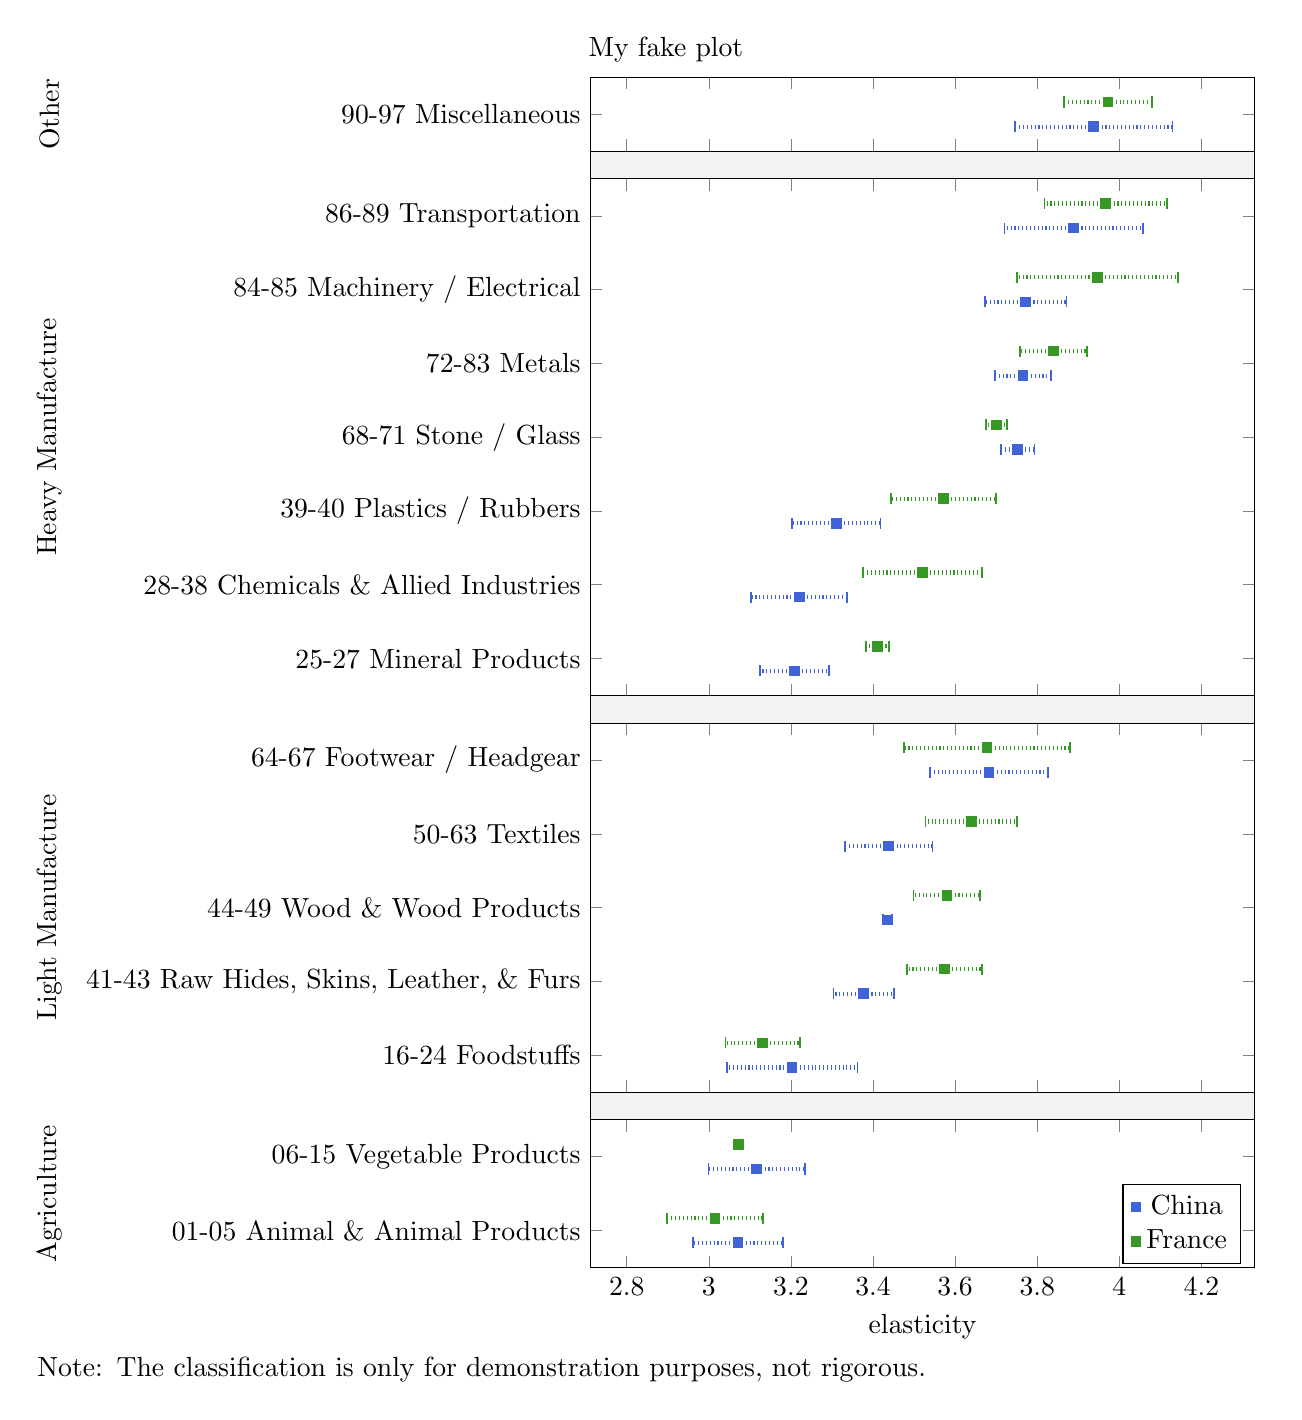
\begin{tikzpicture}
\begin{groupplot}[group style={group size={1 by 4}, x descriptions at={edge bottom}, xlabels at={edge bottom}, vertical sep={10pt}}, xmin={2.711472596269049}, xmax={4.329482058641058}, xlabel={elasticity}, xlabel style={}]
    \nextgroupplot[xticklabel style={}, yticklabel style={}, width={240pt}, height={26.666666666666668pt}, legend style={at={(0.98, 0.02)}, anchor={south east}}, symbolic y coords={90-97  Miscellaneous}, ytick={90-97  Miscellaneous}, ymin={{[normalized]-0.5}}, ymax={{[normalized]0.5}}, scale only axis]
    \addplot[only marks, mark={square*}, mark options={mark size={1.75pt}, line width={0pt}, fill={rgb,255: red, 64; green, 99; blue, 216}, fill opacity={1}, draw={rgb,255: red, 64; green, 99; blue, 216}, draw opacity={1}}, error bars/error mark={|}, error bars/error mark options={mark size={2.0pt}, solid, line width={0.6pt}, fill={rgb,255: red, 64; green, 99; blue, 216}, fill opacity={1}, draw={rgb,255: red, 64; green, 99; blue, 216}, draw opacity={1}}, error bars/error bar style={draw={rgb,255: red, 64; green, 99; blue, 216}, draw opacity={1}, densely dotted, line width={1.5pt}}, draw={rgb,255: red, 64; green, 99; blue, 216}, draw opacity={1}, line width={0.5pt}, error bars/x dir={both}, error bars/x explicit, y filter/.code={{\pgfmathadd{\pgfmathresult}{-0.16666666666666666}}}]
        coordinates {
            (3.937784287258247,90-97  Miscellaneous) +- (0.19179,0)
        }
        ;
    \addplot[only marks, mark={square*}, mark options={mark size={1.75pt}, line width={0pt}, fill={rgb,255: red, 56; green, 152; blue, 38}, fill opacity={1}, draw={rgb,255: red, 56; green, 152; blue, 38}, draw opacity={1}}, error bars/error mark={|}, error bars/error mark options={mark size={2.0pt}, solid, line width={0.6pt}, fill={rgb,255: red, 56; green, 152; blue, 38}, fill opacity={1}, draw={rgb,255: red, 56; green, 152; blue, 38}, draw opacity={1}}, error bars/error bar style={draw={rgb,255: red, 56; green, 152; blue, 38}, draw opacity={1}, densely dotted, line width={1.5pt}}, draw={rgb,255: red, 56; green, 152; blue, 38}, draw opacity={1}, line width={0.5pt}, error bars/x dir={both}, error bars/x explicit, y filter/.code={{\pgfmathadd{\pgfmathresult}{0.16666666666666666}}}]
        coordinates {
            (3.9721360824554686,90-97  Miscellaneous) +- (0.10692,0)
        }
        ;
    \nextgroupplot[xticklabel style={}, yticklabel style={}, width={240pt}, height={186.66666666666666pt}, legend style={at={(0.98, 0.02)}, anchor={south east}}, symbolic y coords={25-27  Mineral Products,28-38  Chemicals \& Allied Industries,39-40  Plastics / Rubbers,68-71  Stone / Glass,72-83  Metals,84-85  Machinery / Electrical,86-89  Transportation}, ytick={25-27  Mineral Products,28-38  Chemicals \& Allied Industries,39-40  Plastics / Rubbers,68-71  Stone / Glass,72-83  Metals,84-85  Machinery / Electrical,86-89  Transportation}, ymin={{[normalized]-0.5}}, ymax={{[normalized]6.5}}, scale only axis]
    \addplot[only marks, mark={square*}, mark options={mark size={1.75pt}, line width={0pt}, fill={rgb,255: red, 64; green, 99; blue, 216}, fill opacity={1}, draw={rgb,255: red, 64; green, 99; blue, 216}, draw opacity={1}}, error bars/error mark={|}, error bars/error mark options={mark size={2.0pt}, solid, line width={0.6pt}, fill={rgb,255: red, 64; green, 99; blue, 216}, fill opacity={1}, draw={rgb,255: red, 64; green, 99; blue, 216}, draw opacity={1}}, error bars/error bar style={draw={rgb,255: red, 64; green, 99; blue, 216}, draw opacity={1}, densely dotted, line width={1.5pt}}, draw={rgb,255: red, 64; green, 99; blue, 216}, draw opacity={1}, line width={0.5pt}, error bars/x dir={both}, error bars/x explicit, y filter/.code={{\pgfmathadd{\pgfmathresult}{-0.16666666666666666}}}]
        coordinates {
            (3.2088295365510877,25-27  Mineral Products) +- (0.08389,0)
            (3.220152632632353,28-38  Chemicals \& Allied Industries) +- (0.11705,0)
            (3.3107441491827307,39-40  Plastics / Rubbers) +- (0.10735,0)
            (3.752248967990113,68-71  Stone / Glass) +- (0.04078,0)
            (3.7655615943371723,72-83  Metals) +- (0.0682,0)
            (3.771895893081587,84-85  Machinery / Electrical) +- (0.09983,0)
            (3.8888937101599996,86-89  Transportation) +- (0.16858,0)
        }
        ;
    \addplot[only marks, mark={square*}, mark options={mark size={1.75pt}, line width={0pt}, fill={rgb,255: red, 56; green, 152; blue, 38}, fill opacity={1}, draw={rgb,255: red, 56; green, 152; blue, 38}, draw opacity={1}}, error bars/error mark={|}, error bars/error mark options={mark size={2.0pt}, solid, line width={0.6pt}, fill={rgb,255: red, 56; green, 152; blue, 38}, fill opacity={1}, draw={rgb,255: red, 56; green, 152; blue, 38}, draw opacity={1}}, error bars/error bar style={draw={rgb,255: red, 56; green, 152; blue, 38}, draw opacity={1}, densely dotted, line width={1.5pt}}, draw={rgb,255: red, 56; green, 152; blue, 38}, draw opacity={1}, line width={0.5pt}, error bars/x dir={both}, error bars/x explicit, y filter/.code={{\pgfmathadd{\pgfmathresult}{0.16666666666666666}}}]
        coordinates {
            (3.4112941179498506,25-27  Mineral Products) +- (0.02765,0)
            (3.5203549937237177,28-38  Chemicals \& Allied Industries) +- (0.14458,0)
            (3.571586377522953,39-40  Plastics / Rubbers) +- (0.12796,0)
            (3.7011158355140754,68-71  Stone / Glass) +- (0.02602,0)
            (3.839621934058071,72-83  Metals) +- (0.08182,0)
            (3.9464532262313834,84-85  Machinery / Electrical) +- (0.19634,0)
            (3.967142768915383,86-89  Transportation) +- (0.14971,0)
        }
        ;
    \nextgroupplot[xticklabel style={}, yticklabel style={}, width={240pt}, height={133.33333333333331pt}, legend style={at={(0.98, 0.02)}, anchor={south east}}, symbolic y coords={16-24  Foodstuffs,41-43  Raw Hides{,} Skins{,} Leather{,} \& Furs,44-49  Wood \& Wood Products,50-63  Textiles,64-67  Footwear / Headgear}, ytick={16-24  Foodstuffs,41-43  Raw Hides{,} Skins{,} Leather{,} \& Furs,44-49  Wood \& Wood Products,50-63  Textiles,64-67  Footwear / Headgear}, ymin={{[normalized]-0.5}}, ymax={{[normalized]4.5}}, scale only axis]
    \addplot[only marks, mark={square*}, mark options={mark size={1.75pt}, line width={0pt}, fill={rgb,255: red, 64; green, 99; blue, 216}, fill opacity={1}, draw={rgb,255: red, 64; green, 99; blue, 216}, draw opacity={1}}, error bars/error mark={|}, error bars/error mark options={mark size={2.0pt}, solid, line width={0.6pt}, fill={rgb,255: red, 64; green, 99; blue, 216}, fill opacity={1}, draw={rgb,255: red, 64; green, 99; blue, 216}, draw opacity={1}}, error bars/error bar style={draw={rgb,255: red, 64; green, 99; blue, 216}, draw opacity={1}, densely dotted, line width={1.5pt}}, draw={rgb,255: red, 64; green, 99; blue, 216}, draw opacity={1}, line width={0.5pt}, error bars/x dir={both}, error bars/x explicit, y filter/.code={{\pgfmathadd{\pgfmathresult}{-0.16666666666666666}}}]
        coordinates {
            (3.202959366517577,16-24  Foodstuffs) +- (0.15913,0)
            (3.377140368378589,41-43  Raw Hides{,} Skins{,} Leather{,} \& Furs) +- (0.07377,0)
            (3.4355209747786595,44-49  Wood \& Wood Products) +- (0.01126,0)
            (3.438321683915909,50-63  Textiles) +- (0.10675,0)
            (3.682790505070825,64-67  Footwear / Headgear) +- (0.14419,0)
        }
        ;
    \addplot[only marks, mark={square*}, mark options={mark size={1.75pt}, line width={0pt}, fill={rgb,255: red, 56; green, 152; blue, 38}, fill opacity={1}, draw={rgb,255: red, 56; green, 152; blue, 38}, draw opacity={1}}, error bars/error mark={|}, error bars/error mark options={mark size={2.0pt}, solid, line width={0.6pt}, fill={rgb,255: red, 56; green, 152; blue, 38}, fill opacity={1}, draw={rgb,255: red, 56; green, 152; blue, 38}, draw opacity={1}}, error bars/error bar style={draw={rgb,255: red, 56; green, 152; blue, 38}, draw opacity={1}, densely dotted, line width={1.5pt}}, draw={rgb,255: red, 56; green, 152; blue, 38}, draw opacity={1}, line width={0.5pt}, error bars/x dir={both}, error bars/x explicit, y filter/.code={{\pgfmathadd{\pgfmathresult}{0.16666666666666666}}}]
        coordinates {
            (3.131025656220859,16-24  Foodstuffs) +- (0.0904,0)
            (3.5743234852783177,41-43  Raw Hides{,} Skins{,} Leather{,} \& Furs) +- (0.09103,0)
            (3.5798621201341323,44-49  Wood \& Wood Products) +- (0.0815,0)
            (3.6395615996802735,50-63  Textiles) +- (0.1118,0)
            (3.677649907599578,64-67  Footwear / Headgear) +- (0.20208,0)
        }
        ;
    \nextgroupplot[xticklabel style={}, yticklabel style={}, width={240pt}, height={53.333333333333336pt}, legend style={at={(0.98, 0.02)}, anchor={south east}}, symbolic y coords={01-05  Animal \& Animal Products,06-15  Vegetable Products}, ytick={01-05  Animal \& Animal Products,06-15  Vegetable Products}, ymin={{[normalized]-0.5}}, ymax={{[normalized]1.5}}, scale only axis]
    \addplot[only marks, mark={square*}, mark options={mark size={1.75pt}, line width={0pt}, fill={rgb,255: red, 64; green, 99; blue, 216}, fill opacity={1}, draw={rgb,255: red, 64; green, 99; blue, 216}, draw opacity={1}}, error bars/error mark={|}, error bars/error mark options={mark size={2.0pt}, solid, line width={0.6pt}, fill={rgb,255: red, 64; green, 99; blue, 216}, fill opacity={1}, draw={rgb,255: red, 64; green, 99; blue, 216}, draw opacity={1}}, error bars/error bar style={draw={rgb,255: red, 64; green, 99; blue, 216}, draw opacity={1}, densely dotted, line width={1.5pt}}, draw={rgb,255: red, 64; green, 99; blue, 216}, draw opacity={1}, line width={0.5pt}, error bars/x dir={both}, error bars/x explicit, y filter/.code={{\pgfmathadd{\pgfmathresult}{-0.16666666666666666}}}]
        coordinates {
            (3.0709577215496724,01-05  Animal \& Animal Products) +- (0.10971,0)
            (3.116792264544351,06-15  Vegetable Products) +- (0.11729,0)
        }
        ;
    \addlegendentry {China}
    \addplot[only marks, mark={square*}, mark options={mark size={1.75pt}, line width={0pt}, fill={rgb,255: red, 56; green, 152; blue, 38}, fill opacity={1}, draw={rgb,255: red, 56; green, 152; blue, 38}, draw opacity={1}}, error bars/error mark={|}, error bars/error mark options={mark size={2.0pt}, solid, line width={0.6pt}, fill={rgb,255: red, 56; green, 152; blue, 38}, fill opacity={1}, draw={rgb,255: red, 56; green, 152; blue, 38}, draw opacity={1}}, error bars/error bar style={draw={rgb,255: red, 56; green, 152; blue, 38}, draw opacity={1}, densely dotted, line width={1.5pt}}, draw={rgb,255: red, 56; green, 152; blue, 38}, draw opacity={1}, line width={0.5pt}, error bars/x dir={both}, error bars/x explicit, y filter/.code={{\pgfmathadd{\pgfmathresult}{0.16666666666666666}}}]
        coordinates {
            (3.0149088492851,01-05  Animal \& Animal Products) +- (0.11674,0)
            (3.072716142092216,06-15  Vegetable Products) +- (0.00286,0)
        }
        ;
    \addlegendentry {France}
\end{groupplot}
\coordinate (freeze) at (current bounding box.west);
\coordinate (title) at (current bounding box.north);
\filldraw[fill=gray, draw=black,fill opacity=0.1] (group c1r2.north west) rectangle (group c1r1.south east);
\filldraw[fill=gray, draw=black,fill opacity=0.1] (group c1r3.north west) rectangle (group c1r2.south east);
\filldraw[fill=gray, draw=black,fill opacity=0.1] (group c1r4.north west) rectangle (group c1r3.south east);
\node[xshift=-1em, rotate=90] at ({freeze}|-{group c1r1.center}) {Other};
\node[xshift=-1em, rotate=90] at ({freeze}|-{group c1r2.center}) {Heavy Manufacture};
\node[xshift=-1em, rotate=90] at ({freeze}|-{group c1r3.center}) {Light Manufacture};
\node[xshift=-1em, rotate=90] at ({freeze}|-{group c1r4.center}) {Agriculture};
\node[yshift=1em] at (title) {My fake plot};
\newdimen\notewidth
                    \pgfextractx{\notewidth}{\pgfpointdiff{\pgfpointanchor{current bounding box}{west}}
                    {\pgfpointanchor{current bounding box}{east}}}\draw node[text width={\the\notewidth}, anchor={north west}, at={(current bounding box.south west)}, align={left}] {Note: The classification is only for demonstration purposes, not rigorous.};
\end{tikzpicture}
\end{document}
